\documentclass[aspectratio=169,10pt]{beamer}
\usetheme{default}
\usecolortheme{seahorse}
\setbeamertemplate{navigation symbols}{}
\setbeamertemplate{footline}[frame number]
\usepackage[T1]{fontenc}
\usepackage{booktabs,graphicx}
\graphicspath{{../../}}
\title{Design Pattern Analysis in a Next.js-Based Video Streaming Application}
\subtitle{23CSE455 Design Patterns --- Case Study, Team A12}
\author{Swaminathan A \and Anna Ouseph \and Leya Paul \and Pooja Sathyan \and Rahul Rajan}
\date{October 2026}
\begin{document}

\begin{frame}\titlepage\end{frame}

\begin{frame}{Application under study}
\begin{columns}[T]
\column{0.42\textwidth}
\small
\begin{itemize}
\item \textbf{netflx-web} (sadmann7), Netflix clone
\item Next.js 13.4 app router, tRPC 10, NextAuth 4, Prisma 4 (MySQL), Stripe, Zustand, React Query, TMDB API
\item Baseline commit \texttt{676e5dd} (2024-06-12)
\item No LICENSE file --- academic analysis only
\item Seven areas: user management, catalogue, subscription, recommendation, authentication, content access, caching
\end{itemize}
\column{0.56\textwidth}
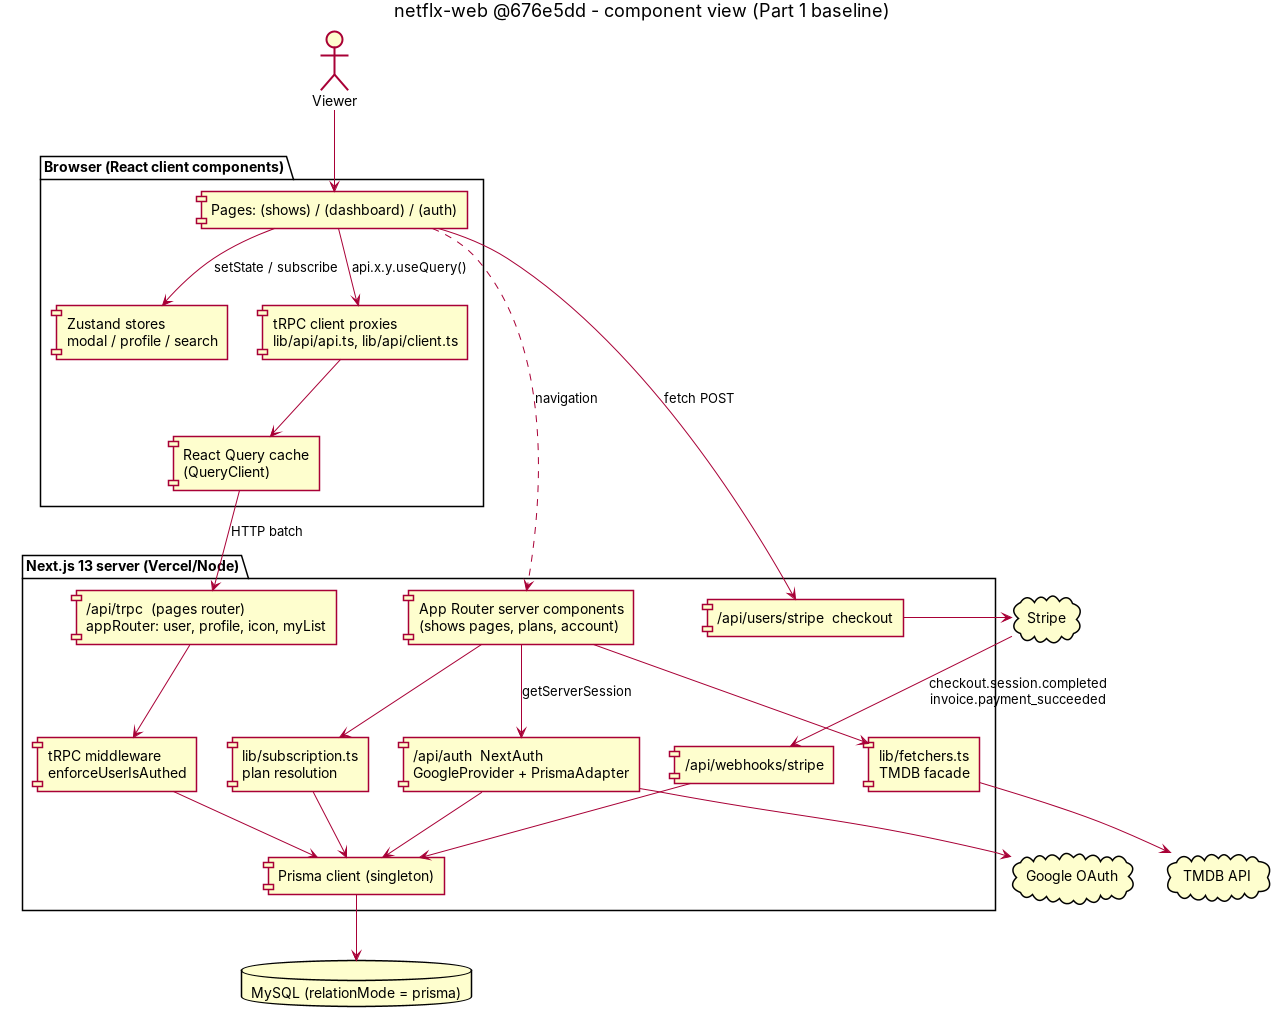
\includegraphics[width=\linewidth]{Part1/diagrams/00_architecture.png}
\end{columns}
\end{frame}

\begin{frame}{Part 1 --- pattern catalogue at the baseline}
\small
\begin{tabular}{@{}llcc@{}}\toprule
Pattern & Instances & \# & Concrete\\\midrule
Chain of Responsibility & Authenticated Procedure Pipeline & 1 & 1\\
Singleton & Shared Prisma Client; Stripe API Client & 2 & 2\\
Observer & Show Modal Selection; Active Profile Selection; Search Results & 3 & 15\\
Decorator & Persisted Profile Store (devtools(persist(\dots))) & 1 & 3\\
Adapter & NextAuth Prisma Persistence Adapter & 1 & 1\\
Strategy & Sign-in Provider Strategy & 1 & 1\\
Facade & TMDB Catalogue Facade & 1 & 1\\
Composite & API Router Tree & 1 & 5\\
Proxy & 2 tRPC client proxies; Environment Secret Guard & 3 & 3\\
Read-Through Cache & My List Query Cache & 1 & 1\\\midrule
\textbf{10 types} & & \textbf{15} & \textbf{33}\\\bottomrule
\end{tabular}
\par\medskip 6 rejected (e.g.\ dead caching proxy, no recommendation logic), 4 uncertain (e.g.\ Stripe webhook). Every range checked by script.
\end{frame}

\begin{frame}{Example: Environment Secret Guard (protection proxy)}
\begin{columns}[T]
\column{0.5\textwidth}\small
\begin{itemize}
\item \texttt{env = new Proxy(parsed.data, \{get\})} in \texttt{env.mjs:92-105}
\item On the client, any non-\texttt{NEXT\_PUBLIC\_} read throws
\item Found on the second review pass (LLM's first answer missed it)
\item Explains a smell found in Part 2: plan data was duplicated because the server list reads secrets
\end{itemize}
\column{0.48\textwidth}
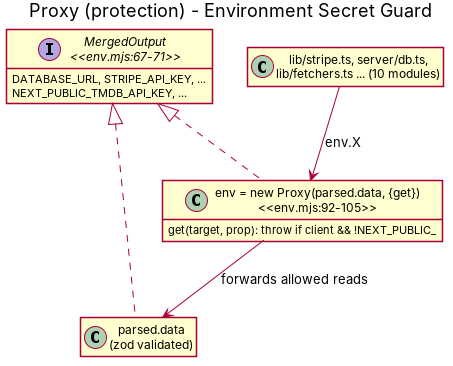
\includegraphics[width=\linewidth]{Part1/diagrams/15_proxy_environment_secret_guard.png}
\end{columns}
\end{frame}

\begin{frame}{Part 2 --- three changes}
\small
\begin{tabular}{@{}p{3.3cm}p{6.6cm}p{3.6cm}@{}}\toprule
Change & What & Tests\\\midrule
CH01 premium + Ultra plan & tier-based premium titles, Ultra (7 profiles), subscription middleware & 29/29\\
CH02 regional restrictions & licences per country, geo header, server-side row filtering & 45/45\\
CH03 parental control & KIDS / TEEN / ADULT rating per profile & 65/65\\\bottomrule
\end{tabular}
\par\medskip
\begin{itemize}
\item Characterization tests written first and run on the \emph{original} code (19/19)
\item New student-added \textbf{Content Access Rule Chain}: Region $\rightarrow$ Maturity $\rightarrow$ Premium (hide before lock)
\item Existing tRPC middleware chain extended with \texttt{attachSubscription}
\end{itemize}
\end{frame}

\begin{frame}{Pattern evolution}
\begin{columns}[T]
\column{0.5\textwidth}\small
\begin{tabular}{@{}lcccc@{}}\toprule
Snapshot & Types & Inst. & Concr.\\\midrule
baseline & 10 & 15 & 33\\
CH01 & 11 & 17 & 37\\
CH02 & 11 & 17 & 39\\
CH03 & 11 & 17 & 42\\\bottomrule
\end{tabular}
\par\medskip
\begin{itemize}
\item New: Content Access Rule Chain (CoR), Access Rule Evaluation Template (Template Method)
\item Extended: auth pipeline, router tree, profile observers
\item Modified: TMDB facade, search observer; none removed
\end{itemize}
\column{0.48\textwidth}
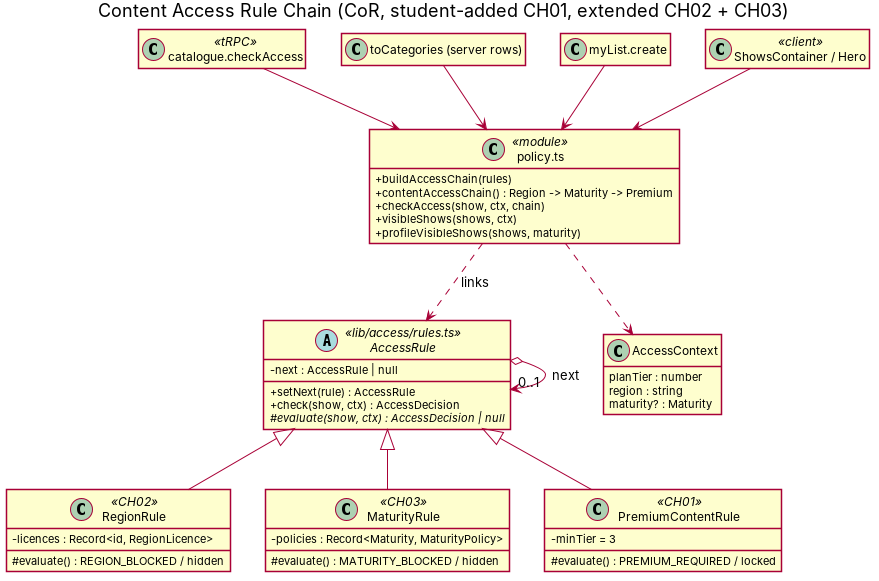
\includegraphics[width=\linewidth]{Part2/diagrams/01_content_access_rule_chain_CH03.png}
\end{columns}
\end{frame}

\begin{frame}{Refactoring --- real smells, measured with the same tool}
\small
\begin{tabular}{@{}p{5.2cm}p{4.2cm}rr@{}}\toprule
Smell & Technique & Before & After\\\midrule
Duplicated plan data (UI vs server, already drifted) & shared client-safe catalogue & 139 NLOC & 123 (+1 plan)\\
Copy-pasted TMDB fetch blocks & rows as data + \texttt{fetchRows} & max CCN 9 & 3\\
Same row array in 3 pages & \texttt{GENRE\_ROWS} + \texttt{toCategories} & 174 NLOC & 116\\
Duplicated zod schema / lookups in My List & Extract Variable / Function & 169 NLOC & 114\\\bottomrule
\end{tabular}
\par\medskip
Whole \texttt{src/}: 6694 $\rightarrow$ 6916 NLOC (+3.3\%), avg CCN 2.31 $\rightarrow$ 2.26. LOC alone does not prove better design; the evidence is behaviour preserved by tests.
\end{frame}

\begin{frame}{Part 3 --- four languages, one shared fixture}
\small
\begin{tabular}{@{}lrrrr@{}}\toprule
 & Java & Python & JavaScript & C++\\\midrule
cases passed (10 problems) & 107/107 & 107/107 & 107/107 & 107/107\\
total source LOC & 497 & 316 & 316 & 558\\
max function CC & 5 & 6 & 5 & 6\\
median process time (ms) & 86.7 & 14.9 & 32.6 & 1.8\\\bottomrule
\end{tabular}
\par\medskip
\begin{itemize}
\item Proxy: JS \texttt{Proxy} trap $\approx$ source; Python \texttt{\_\_getattr\_\_}; Java \texttt{reflect.Proxy}; C++ plain class
\item JS needs no classes for Observer / Decorator / Adapter (functions and object literals, like zustand and next-auth)
\item Times are start-up dominated; \texttt{dataclasses} import costs $\approx$20--26\,ms in Python
\end{itemize}
\end{frame}

\begin{frame}{LLM use and verification}
\small
\begin{itemize}
\item One Claude (Opus 5.5) session for Parts 1--3; prompts, outputs and claim tables in \texttt{Part*/llm/}, summary in \texttt{data/llm.csv}
\item Errors found by checking: missed instance (env proxy), 3 wrong line ranges, NLOC first measured without \texttt{.tsx}, a max-CCN rise that was a lizard artefact
\item Not accepted: Stripe webhook as Observer (kept uncertain)
\item All generated code is covered by tests (65 app tests, 428 cross-language checks)
\end{itemize}
\end{frame}

\begin{frame}{Findings}
\small
\begin{itemize}
\item Most patterns are inherited from frameworks (tRPC, zustand, NextAuth, React Query) and configured, not written
\item Recommendation has no pattern because it has no logic
\item A chain of rules absorbed premium, region and parental control with one class each
\item Pre-existing issues: client-side PIN check, missing ownership checks on profile / My List, dead caching proxy, two parallel tRPC clients
\item Limits: no end-to-end run with real Stripe / TMDB / Google; sample licence data
\end{itemize}
\end{frame}

\end{document}
